\section{Choosing the Framework}
As it was explained in the previous chapter, there are a lot of agent based frameworks, yet most of them are designed for a narrow set of tasks. To choose the framework correctly one should know what features one need in the multi-agent system. Each feature or concept can be either provided by an operational system, by a programming language, by a 3rd party library or by a framework itself (Figure~\ref{Feature}).
 \begin{figure}[h!]
    \begin{center}
      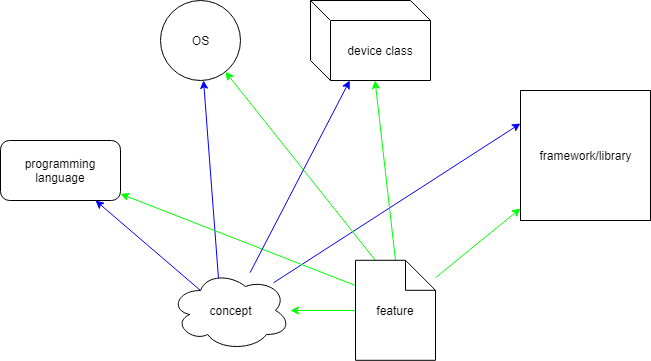
\includegraphics[width=300pt]{feature_dependencies}
      \caption{Possible feature containers.}
      \label{Feature}
     \end{center}
    \end{figure}

By looking through the frameworks it can be seen that some of them are implemented for multiple programming languages. Most of the languages (like C++, Java or Python) are cross-platform.
To sum up, it is almost possible to choose the language, the framework and the platform separately.
Nevertheless, after a closer look on the implementations, it became clear that most framework ports on other languages are either poorly made or already abandoned.
In addition, each framework included some mechanisms that were redundant when applied to the chosen task. Usually, agents were either automatically provisioned with individual threads or were executed by some non-configurable custom scheduler. For some of the frameworks it was hardly possible to find any readable documentation, therefore their learning curve was far from being optimal.  After comparison was made JADE Java framework was selected.

 The main reasons to choose it were speed \cite{JAVAap} (for there are no nondetachable visualization or control mechanisms involved), extensible documentation (mostly gathered on their official site \cite{jadeDoc}, especially \cite{jadeBook}), alive community and FIPA-compliance \cite{ap3}. Other than that it does feature some tools for debugging and visualization of the created system that may simplify the future development. Of course there is a point where the system specification of the system goes beyond the JADE agent approach but using JADE will be plausible to create the test version of the framework, where the efficiency of the end product is of no concern.

